\documentclass[11pt,a4paper]{article}

\usepackage[T1]{fontenc}
\usepackage[utf8]{inputenc}
\usepackage{lmodern}
\usepackage{microtype}
\usepackage[a4paper,top=29mm,bottom=30mm,left=30mm,right=30mm]{geometry}
\usepackage{amsmath,amssymb,mathtools,amsthm}
\usepackage{bm}
\usepackage{booktabs}
\usepackage{enumitem}
\usepackage{authblk}
\usepackage{tikz}
\usetikzlibrary{arrows.meta,positioning,shapes.geometric}
\usepackage[numbers,sort&compress]{natbib}
\usepackage{xcolor}
\usepackage{hyperref}
\usepackage[nameinlink,noabbrev]{cleveref}

\input{glyphtounicode}
\pdfgentounicode=1
\hypersetup{
  colorlinks=true,
  linkcolor=blue!45!black,
  citecolor=blue!45!black,
  urlcolor=blue!45!black,
  pdftitle={Quantum screening jets and deformation intertwiners for the symmetric Carrollian W3-algebra},
  pdfauthor={Shubham Kumar},
  pdfsubject={Carrollian conformal field theory, W-algebras, screening operators and flat-space holography},
  pdfkeywords={Carrollian W-algebra, screening charge, Miura transformation, deformation intertwiner, flat-space holography}
}

\setcounter{tocdepth}{2}
\setlength{\parindent}{1.25em}
\setlength{\parskip}{0pt}
\linespread{1.10}
\setlist{nosep,leftmargin=2em}
\allowdisplaybreaks[2]
\numberwithin{equation}{section}

\newtheorem{theorem}{Theorem}[section]
\newtheorem{lemma}[theorem]{Lemma}
\newtheorem{proposition}[theorem]{Proposition}
\newtheorem{corollary}[theorem]{Corollary}
\theoremstyle{remark}
\newtheorem{remark}[theorem]{Remark}

% arXiv TeX Live 2025 compatibility for cleveref theorem-like environments.
\AddToHook{env/theorem/begin}{\crefalias{section}{theorem}}
\AddToHook{env/lemma/begin}{\crefalias{section}{lemma}}
\AddToHook{env/proposition/begin}{\crefalias{section}{proposition}}
\AddToHook{env/corollary/begin}{\crefalias{section}{corollary}}
\AddToHook{env/remark/begin}{\crefalias{section}{remark}}

\newcommand{\Car}{\mathrm{Car}}
\newcommand{\Av}[1]{\operatorname{Av}\!\left(#1\right)}
\newcommand{\Sing}{\operatorname{Sing}}
\newcommand{\Res}{\operatorname*{Res}}
\newcommand{\LRes}{\operatorname*{LRes}}
\newcommand{\Coeff}{\operatorname{Coeff}}
\newcommand{\Hom}{\operatorname{Hom}}
\newcommand{\ad}{\operatorname{ad}}
\newcommand{\PBW}{\mathrm{PBW}}
\newcommand{\cl}{\mathrm{cl}}
\newcommand{\T}{\mathrm{T}}
\newcommand{\ii}{\mathrm{i}}
\newcommand{\dd}{\mathrm{d}}
\newcommand{\cU}{\mathcal U}
\newcommand{\cA}{\mathcal A}
\newcommand{\cB}{\mathcal B}
\newcommand{\cS}{\mathcal S}
\newcommand{\wideF}{\widehat{\mathcal F}}
\newcommand{\wideP}{\widehat{\mathcal P}}
\newcommand{\eps}{\varepsilon}

\title{\bfseries Quantum screening jets and deformation\\[1mm]
intertwiners for the symmetric\\[1mm]
Carrollian $W_3$-algebra}

\author[1,2]{Shubham Kumar}
\affil[1]{Institut f\"ur Physik, Mathematische Physik, Johannes Gutenberg-Universit\"at Mainz,
Staudingerweg 7, 55128 Mainz, Germany}
\affil[2]{University of Maryland Global Campus Europe, Wiesbaden, Germany}
\date{}

\begin{document}
\maketitle
\vspace{-1.5em}
\begin{center}
\small\href{mailto:skumar@students.uni-mainz.de}{skumar@students.uni-mainz.de},
\href{mailto:shubham.kumar@faculty.umgc.edu}{shubham.kumar@faculty.umgc.edu}
\end{center}

\begin{abstract}
We construct the simple-root quantum screening jets of the proper symmetric Carrollian
$W_3$-algebra obtained from the contracted Miura transformation.  For each simple root, the
two relativistic Fateev--Lukyanov screening families contract to one such jet.  Its leading coefficients
$Q_i^{[0]}$ are finite, non-zero intertwiners on completed horizontal Fock families and screen
the spin-two and primary spin-three generators precisely on $\alpha^+\mu=1$.  The parent
reciprocity $\beta_+\beta_-=-4$ becomes $\alpha^+\beta_1=-2$: one branch remains a local
screening, whereas the reciprocal branch is absorbed into the background charge.  The first
relative coefficients are also finite and non-zero, but their target representations have
different first tangents.  In a fixed PBW frame the canonical coefficients $Q_i^{[1]}$ therefore
satisfy an inhomogeneous deformation-intertwiner equation, rather than an ordinary commutant
relation.  We verify its nonlinear spin-three form directly from the two finite-parent
orderings; their average supplies a fixed contact term, and no additional counterterm is
introduced.  Finally, on the gravity branch $\alpha^-=0$, $\alpha^+=\ii a_s$, we establish the
semiclassical dictionary to flat higher-spin gravity.  The bulk leading and barred-linear
Noether charges realize $Q_i^{[0],\cl}$ and the raw coefficient
$\widetilde Q_i^{[1],\cl}$; the canonical $Q_i^{[1]}$ is the corresponding PBW
covariantization and is not an ordinary second screening.
\end{abstract}

\tableofcontents

\section{Introduction}
\label{sec:introduction}

Free-field realizations organize the nonlinear structure of two-dimensional $W$-algebras
\cite{Zamolodchikov} in
a form adapted to both representation theory and Coulomb-gas methods.  In the relativistic
theory, the quantum Miura transformation packages the currents into an ordered differential
operator, while screening charges intertwine Fock modules and characterize the $W$-currents
through commutant conditions \cite{DotsenkoFateev,FateevLukyanov,Felder,BouwknegtSchoutens,
FeiginFrenkel,LitvinovSpodyneiko,TsuchiyaKanie,BalogEtAl}.  It is therefore natural to ask
what survives under a Carrollian contraction.

For three-dimensional flat holography, this question is particularly concrete.  The asymptotic
symmetry algebra contains $\mathfrak{bms}_3$, interpreted as a conformal Carroll algebra
\cite{BarnichCompere,DuvalGibbonsHorvathy,Ruzziconi}.  Fredenhagen and H\"orl
constructed proper symmetric quantum Carrollian $W_N$-algebras by contracting two
relativistic Miura operators \cite{FredenhagenHoerl}.  The reversal of the barred polarization
forces a symmetric average of the two parent orderings; with that prescription, the basic
structure constants retain their classical form; earlier free-field realizations of
$\mathfrak{bms}_3$ and its extensions were studied in \cite{BanerjeeJatkarMukhiNeogi}.
Building on the Brown--Henneaux analysis, $W$-algebras arise as asymptotic symmetries in
AdS$_3$ higher-spin gravity
\cite{BrownHenneaux,HenneauxRey,CampoleoniFredenhagenPfenningerTheisen}, while their flat spin-three
counterparts and flat higher-spin phases were developed in
\cite{AfsharEtAl,GonzalezEtAl,AmmonEtAl}; see
\cite{CampoleoniFredenhagenBook} for a systematic account.  Independently, D'Arcy, Delfante and
Fredenhagen derived a classical Carrollian Coulomb gas from asymptotically flat higher-spin
Chern--Simons gravity in a flat diagonal gauge \cite{DArcyDelfanteFredenhagen}.  Its residual
pure-gauge transformations are generated by Carrollian Noether screenings, and its
gauge-invariant observables are row-determinant Miura combinations, paralleling free-field
variables used in higher-spin quantization \cite{CampoleoniFredenhagenRaeymaekers}.  Together with the
analysis of Carrollian quantum states in \cite{FredenhagenProhazkaTiefenbacher}, these results
leave a sharply defined missing step: the simple-root quantum screening jets for the proper
symmetric Carrollian construction.

We address this problem for $N=3$, the first nonlinear case.  Three features distinguish the
answer from the relativistic template.

First, the two roots of the relativistic screening equation obey
$\beta_+\beta_-=-4$.  A regular Carrollian local limit keeps one branch with
$\beta=\eps\beta_1+O(\eps^3)$; the reciprocal branch diverges and fixes the contracted
background charge.  The remnant of the two-branch relation is therefore
\begin{equation}
  \alpha^+\beta_1=-2,
  \qquad \beta_1=-2\mu,
  \qquad \alpha^+\mu=1.
  \label{eq:intro-locus}
\end{equation}
There is only one regular local leading screening per simple root.

Second, the unbarred and barred parent charges contract to a jet rather than to two independent
screenings.  The leading coefficient is an ordinary screening.  The first relative coefficient
compares intertwiners whose target Fock momenta follow different curves.  In a common PBW-flat
frame it is a deformation intertwiner,
\begin{equation}
  Q_i^{[1]}=\widetilde Q_i^{[1]}-\mathsf A_{\T,i}Q_i^{[0]},
  \qquad
  \mathsf A_{\T,i}=\mu\,\alpha_i\!\cdot q^-+\nu\,\alpha_i\!\cdot q^+,
  \qquad \nu=-\alpha^-\mu^2,
  \label{eq:intro-covariantization}
\end{equation}
and obeys
\begin{equation}
 [Q_i^{[1]},\cU_{3,n}^{\sigma,[0]}]_{\PBW}
 +\frac12\,\Delta\cU_{\T,3,n}^{\sigma,[1]}Q_i^{[0]}=0,
 \qquad i=1,2,\quad \sigma=\pm.
 \label{eq:intro-main}
\end{equation}
The inhomogeneous term is the connection required to compare the moving target
representations; it is not removable by a scalar choice of scheme.

Third, the same distinction has a semiclassical bulk realization.  The leading bulk Noether
charges match $Q_i^{[0],\cl}$ and the barred-linear charges match the raw moving-frame
coefficient $\widetilde Q_i^{[1],\cl}$.  Passing to a fixed boundary target frame produces
\cref{eq:intro-covariantization}.  Thus the bulk does not supply an ordinary second quantum
screening.

\begin{figure}[t]
\centering
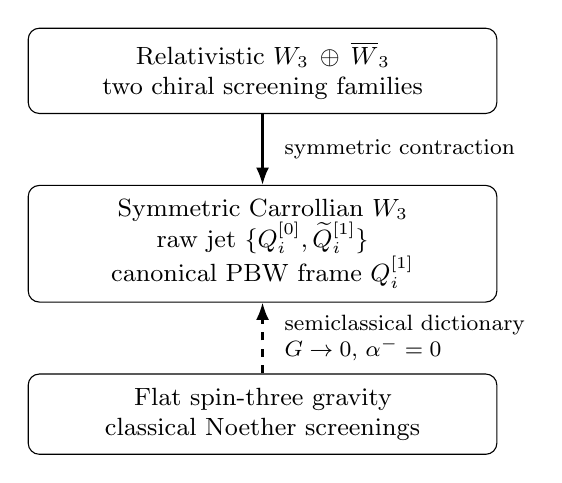
\begin{tikzpicture}[
  node distance=9mm,
  box/.style={draw,rounded corners,align=center,inner sep=5pt,text width=56mm,font=\small},
  arr/.style={-{Latex[length=2.2mm]},thick},
  darr/.style={-{Latex[length=2.2mm]},thick,dashed}
]
\node[box] (parent) {Relativistic $W_3\oplus\overline W_3$\\two chiral screening families};
\node[box,below=of parent] (jet) {Symmetric Carrollian $W_3$\\raw jet $\{Q_i^{[0]},\widetilde Q_i^{[1]}\}$\\canonical PBW frame $Q_i^{[1]}$};
\node[box,below=of jet] (bulk) {Flat spin-three gravity\\classical Noether screenings};
\draw[arr] (parent) -- node[right,xshift=1.5mm,font=\footnotesize]{symmetric contraction} (jet);
\draw[darr] (bulk) -- node[right,xshift=1.5mm,font=\footnotesize,align=left]{semiclassical dictionary\\$G\to0$, $\alpha^-=0$} (jet);
\end{tikzpicture}
\caption{The parent systems contract to a raw screening jet; its fixed-target representative
is the canonical deformation intertwiner $Q_i^{[1]}$.  The bulk charges realize the leading
and raw semiclassical coefficients.}
\label{fig:structure}
\end{figure}

The leading theorem gives the inclusion
\begin{equation}
  W_3^{\Car}\subseteq \bigcap_{i=1}^{2}\ker\!\left(\ad Q_i^{[0]}\right)
  \label{eq:kernel-inclusion}
\end{equation}
as an identity of intertwiners on the Fock families specified below.  Equality is not proved.
Here $\ad Q_i^{[0]}$ denotes the source--target intertwiner differential
$U_{\T}Q_i^{[0]}-Q_i^{[0]}U_{\rm S}$, rather than an adjoint action in a single
endomorphism algebra.
We likewise make no claim that the two jet coefficients form a pair of ordinary quantum
screenings, nor do we claim screening--screening closure, Serre relations, a BRST or Felder
complex, or a quantum-group structure.  The distinction
between $\widetilde Q_i^{[1]}$ and $Q_i^{[1]}$ is maintained throughout.

The paper is organized as follows.  \Cref{sec:free-fields} fixes the crossed free fields,
averaged ordering and primary $W_3$ currents.  \Cref{sec:parent-leading} derives the parent
screening condition, its reciprocal branch, the contracted parameter hierarchy and the leading
operator theorem.  \Cref{sec:jet} constructs the finite screening jet and exhibits the $A_1$
obstruction.  \Cref{sec:nonlinear} proves the nonlinear deformation-intertwiner equation by
both finite-parent contraction and a direct averaged-order OPE.  \Cref{sec:bulk} establishes
the semiclassical bulk dictionary.  Technical formulas and normalization notes are collected in
the appendices.

\section{Symmetric Carrollian free fields and primary \texorpdfstring{$W_3$}{W3} currents}
\label{sec:free-fields}

\subsection{Crossed Heisenberg algebra, potentials and ordering}

Let
\begin{equation}
 \mathfrak h=\left\{x\in\mathbb C^3\,\middle|\,\sum_{a=1}^3x_a=0\right\},
 \qquad \kappa_{ab}=\delta_{ab}-\frac13,
 \label{eq:kappa}
\end{equation}
and choose the simple roots
\begin{equation}
 \alpha_1=(1,-1,0),\qquad \alpha_2=(0,1,-1),\qquad
 \alpha_i\!\cdot\alpha_j=A_{ij},\qquad
 A=\begin{pmatrix}2&-1\\-1&2\end{pmatrix}.
 \label{eq:roots}
\end{equation}
The symmetric Carrollian currents $P_a=J_a^+$ and $N_a=J_a^-$ satisfy
\begin{equation}
 P_a(z)P_b(w)\sim0,\qquad N_a(z)N_b(w)\sim0,\qquad
 N_a(z)P_b(w)\sim\frac{\kappa_{ab}/2}{(z-w)^2},
 \label{eq:crossed-heisenberg}
\end{equation}
with $\sum_aP_a=\sum_aN_a=0$.  Introducing $P_a=\partial\varphi_a^+$ and
$N_a=\partial\varphi_a^-$ fixes
\begin{equation}
 \varphi_a^-(z)\varphi_b^+(w)\sim \frac{\kappa_{ab}}2\log(z-w),
 \qquad
 [p_a^-,q_b^+]=[p_a^+,q_b^-]=\frac{\kappa_{ab}}2.
 \label{eq:potential-ope}
\end{equation}
The plus sign in \cref{eq:potential-ope} follows from the parent convention
$J_a(z)J_b(w)\sim\kappa_{ab}(z-w)^{-2}$ when $J_a=\partial\varphi_a$.  Relative to a
canonically normalized real boson, $\varphi=\ii\phi_{\rm real}$; this real-form rotation is
responsible for the imaginary background charge on the gravity branch.

For later use it is important that the crossed algebra is not merely the limiting algebra of
the contraction.  If $a_{a,n}$ and $\bar a_{a,n}$ are the modes of the two parent Heisenberg
systems, with
\begin{equation}
 [a_{a,m},a_{b,n}]=m\kappa_{ab}\delta_{m+n,0},\qquad
 [\bar a_{a,m},\bar a_{b,n}]=m\kappa_{ab}\delta_{m+n,0},
 \label{eq:parent-heisenberg}
\end{equation}
then the ultrarelativistic, equal-time embedding is
\begin{equation}
 P_{a,n}=\frac{\eps}{2}\bigl(a_{a,n}+\bar a_{a,-n}\bigr),\qquad
 N_{a,n}=\frac{1}{2\eps}\bigl(a_{a,n}-\bar a_{a,-n}\bigr).
 \label{eq:mode-contraction}
\end{equation}
The reversal of the barred mode changes the sign of its central term, and direct substitution
gives
\begin{equation}
 [P_{a,m},P_{b,n}]=[N_{a,m},N_{b,n}]=0,\qquad
 [N_{a,m},P_{b,n}]=\frac m2\kappa_{ab}\delta_{m+n,0}
 \label{eq:finite-eps-crossed}
\end{equation}
for every $\eps\ne0$.  With $t=\eps^2$, the parent Weyl embeddings are
understood after scalar extension to $\mathbb C((t^{1/2}))$; the contracted currents and the
transported screening vertices considered below lie in the regular $t$-adic subcategory over
$\mathbb C[[t]]$.  Thus the crossed Heisenberg brackets themselves are $\eps$-independent;
the remaining contraction data reside in the composite Miura fields, background charges and
parent vertex embeddings.  This exact finite-$\eps$ statement is what permits the
parent screening relations to be transported before coefficient extraction; it also prevents
the opposite parent polarizations from being identified prematurely.

Products containing one $N$-field use the symmetric ordering inherited from the two parent
polarizations,
\begin{equation}
 \Av{N P_1\cdots P_r}
 :=\frac12\left(:N P_1\cdots P_r:+:P_1\cdots P_r N:\right).
 \label{eq:averaged-order}
\end{equation}
This is not a freely chosen limiting convention: it is obtained by retaining the two parent
normal-order orientations until after coefficient extraction \cite{FredenhagenHoerl}.

\subsection{Contracted Miura currents}

For three traceless parent currents $X_a$, define the ordered row-determinant
\begin{equation}
 \mathcal R(X,a)=\prod_{j=1}^3(a\partial-X_j)
 =(a\partial)^3-u_2(a\partial)-u_3,
 \qquad
 w(X,a):=u_3-\frac a2\partial u_2.
 \label{eq:parent-miura}
\end{equation}
The symmetric contraction embeds the two parent orientations, for $t=\eps^2$, as
\begin{equation}
 X_a^{\rm u}=\eps^{-1}P_a+\eps N_a,\quad
 a_{\rm u}=\eps^{-1}\alpha^++\eps\alpha^-,
 \qquad
 X_a^{\rm b}=\eps^{-1}P_a-\eps N_a,\quad
 a_{\rm b}=\eps^{-1}\alpha^+-\eps\alpha^-.
 \label{eq:parent-embeddings}
\end{equation}
After the barred equal-time map,
\begin{equation}
 \mathbb W^+(t)=\frac{\eps^3}{2}(w_{\rm u}+w_{\rm b}),\qquad
 \mathbb W^-(t)=\frac{\eps}{2}(w_{\rm u}-w_{\rm b}).
 \label{eq:contracted-primary-families}
\end{equation}
Parity under $(N,\alpha^-)\mapsto(-N,-\alpha^-)$ gives
\begin{equation}
 \mathbb W^+(t)=\cU_3^++t^2\cU_{3,+}^{(2)},\qquad
 \mathbb W^-(t)=\cU_3^-+t^2\cU_{3,-}^{(2)}.
 \label{eq:no-universal-linear-term}
\end{equation}
The universal primaries have no coefficient of order $t$; their represented actions on moving
Fock modules need not share this property.

In the reduced variables $P_3=-P_1-P_2$ and $N_3=-N_1-N_2$, the spin-two fields are
\begin{align}
 U_2^+&=P_1^2+P_1P_2+P_2^2-\alpha^+(2P_1'+P_2'),
 \label{eq:U2plus}\\
 U_2^-&=2\Av{N_1P_1}+\Av{N_1P_2}+\Av{N_2P_1}+2\Av{N_2P_2}
 \nonumber\\[-1mm]
 &\hspace{13mm}-\alpha^+(2N_1'+N_2')-\alpha^-(2P_1'+P_2').
 \label{eq:U2minus}
\end{align}
The primary spin-three fields are
\begin{align}
 \cU_3^+={}&-P_1^2P_2-P_1P_2^2
 +\alpha^+\left(\frac32P_1P_2'+\frac12P_1'P_2+P_2P_2'\right)
 -\frac{(\alpha^+)^2}{2}P_2'',
 \label{eq:U3plus}\\
 \cU_3^-={}&-2\Av{N_1P_1P_2}-\Av{N_1P_2^2}-\Av{N_2P_1^2}
 -2\Av{N_2P_1P_2}
 \nonumber\\
 &+\alpha^-\left(\frac32P_1P_2'+\frac12P_1'P_2+P_2P_2'\right)
 \nonumber\\
 &+\alpha^+\Bigl(\frac32\Av{N_1P_2'}+\frac12\Av{N_1'P_2}
 +\frac12\Av{N_2P_1'}+\Av{N_2P_2'}
 \nonumber\\[-1mm]
 &\hspace{29mm}+\frac32\Av{N_2'P_1}+\Av{N_2'P_2}\Bigr)
 \nonumber\\
 &-\alpha^+\alpha^-P_2''-\frac{(\alpha^+)^2}{2}N_2''.
 \label{eq:U3minus}
\end{align}
The second field is the directional derivative of the first under
$(P,\alpha^+)\mapsto(P+sN,\alpha^++s\alpha^-)$ at $s=0$.  It therefore contains at most
one $N$-field.  Together with \cref{eq:crossed-heisenberg}, this one-$N$ filtration bounds the
number of Wick contractions in every screening OPE below.

\section{Parent screenings and leading Carrollian charges}
\label{sec:parent-leading}

\subsection{Parent screening equation and the reciprocal branch}

For a parent simple-root vertex $V_i=:e^{\lambda\alpha_i\cdot\varphi}:$, its spin-two weight
in the conventions of \cref{eq:parent-miura} is
\begin{equation}
 h(\lambda\alpha_i)=\lambda^2+a\lambda.
 \label{eq:parent-weight}
\end{equation}
Thus the parent screening locus is
\begin{equation}
 a\lambda+\lambda^2=1.
 \label{eq:parent-screening-locus}
\end{equation}
In the $A_1$ single-field normalization
$\varphi_{\rm sf}^{\pm}=-\alpha_1\cdot\varphi^{\pm}/2$ and $\beta=-2\lambda$, this becomes
\begin{equation}
 \beta^2-2a\beta-4=0,
 \qquad \beta_+\beta_-=-4,
 \qquad \beta_++\beta_-=2a.
 \label{eq:reciprocal-parent}
\end{equation}
Writing $\beta_+=2b$ and $\beta_-=-2/b$ gives $a=b-b^{-1}$.  Thus the two roots are the
usual reciprocal Coulomb-gas momenta, expressed in the real form selected by
\cref{eq:potential-ope}.  The product relation, rather than the individual parametrization,
is the invariant datum that survives the contraction.
The same locus screens the parent spin-three primary.  For $A_2$ this follows directly from
the ordered Miura OPE: the non-derivative residue factorizes by
$a\lambda+\lambda^2-1$, and on \cref{eq:parent-screening-locus} the singular parts are total
derivatives.  In reduced variables $X_3=-X_1-X_2$, explicit witnesses are
\begin{align}
 \Sing[u_2(z)V_i(w)]&=\partial_w\left(\frac{V_i(w)}{z-w}\right),
 \qquad i=1,2,
 \label{eq:parent-u2-witness}\\
 \Sing[u_3(z)V_1(w)]&=\partial_w\left(
 \frac{(X_1+X_2)V_1(w)}{z-w}\right),
 \label{eq:parent-u3-root1}\\
 \Sing[u_3(z)V_2(w)]&=\partial_w\left(
 -\frac{aV_2(w)}{(z-w)^2}-\frac{X_1V_2(w)}{z-w}\right).
 \label{eq:parent-u3-root2}
\end{align}
These formulas hold on \cref{eq:parent-screening-locus} and are the finite objects contracted in
\cref{sec:nonlinear}; no higher-rank extrapolation is needed for the present theorem.

Take a regular single-field branch
\begin{equation}
 \beta=\eps\beta_1+\eps^3\beta_3+O(\eps^5),\qquad
 \bar\beta=\eps\beta_1+\eps^3\bar\beta_3+O(\eps^5),
 \label{eq:beta-expansions}
\end{equation}
and $a=\eps^{-1}\alpha^++\eps\alpha^-$,
$\bar a=\eps^{-1}\alpha^+-\eps\alpha^-$.  Expanding
\cref{eq:reciprocal-parent} gives
\begin{equation}
 \alpha^+\beta_1=-2,\qquad
 \alpha^+\beta_3=\frac12\beta_1^2-\alpha^-\beta_1,\qquad
 \alpha^+\bar\beta_3=\frac12\beta_1^2+\alpha^-\beta_1.
 \label{eq:single-field-hierarchy}
\end{equation}
Equivalently, in the root normalization $\beta_1=-2\mu$,
\begin{equation}
 \alpha^+\mu=1,\qquad
 \mu_3=-\mu^3-\alpha^-\mu^2,\qquad
 \bar\mu_3=-\mu^3+\alpha^-\mu^2,\qquad
 \nu:=\frac{\mu_3-\bar\mu_3}{2}=-\alpha^-\mu^2.
 \label{eq:root-hierarchy}
\end{equation}
The leading equation can also be obtained without referring back to the parent quadratic.
In the $A_1$ normalization $[J_m^+,J_n^-]=m\delta_{m+n,0}/4$, set
\begin{equation}
 M=2:J^+J^+:+2\alpha^+\partial J^+,\qquad
 L=4\Av{J^+J^-}+2\alpha^+\partial J^-+2\alpha^-\partial J^+.
 \label{eq:A1-spin-two-fields}
\end{equation}
For $E=:e^{\beta_1\varphi^+}:$, the plus field has no contraction with the exponent, and a
single crossed contraction gives
\begin{equation}
 M(z)E(w)\sim0,\qquad
 L(z)E(w)\sim-\frac{\alpha^+\beta_1}{2}\frac{E(w)}{(z-w)^2}
 +\frac{\partial E(w)}{z-w}.
 \label{eq:contracted-spin-two-check}
\end{equation}
Consequently the weight-one condition is again $\alpha^+\beta_1=-2$.  The parent expansion
and the contracted OPE are independent derivations: the former retains the reciprocal branch,
whereas the latter shows directly that the leading relation is an exact quantum condition and
does not depend on the averaged ordering.

The reciprocal parent solution $-4/\beta$ diverges as $\eps^{-1}$, and
\begin{equation}
 \alpha^+=\lim_{\eps\to0}\eps a=-\frac{2}{\beta_1}.
 \label{eq:reciprocity-limit}
\end{equation}
Hence the second parent branch does not give a second regular local leading density; its
information is retained in the background charge.

For $A_2$ the counting is therefore
\begin{equation}
 2\ \text{simple roots}\times1\ \text{regular branch}\times2\ \text{jet coefficients}=4,
 \label{eq:screening-count}
\end{equation}
matching the two exponential and two barred-linear elementary bulk charges encountered in
\cref{sec:bulk}.  On the gravity branch $c_L=0$, $c_M\ne0$ implies $\alpha^-=0$ and
$\alpha^+\ne0$; then $\nu=0$, so the strict tangent density is purely
$:(\mu\alpha_i\cdot\varphi^-)E_i:$, exactly the field content required by the barred-linear
bulk charges.  We keep $\alpha^-$ arbitrary until the bulk comparison because the quantum
Carrollian algebra and the deformation-intertwiner theorem exist away from this locus.

\subsection{Carrier, non-vanishing and the leading theorem}

For each simple root define
\begin{equation}
 E_i(z)=:\!\exp\!\bigl(\mu\alpha_i\cdot\varphi^+(z)\bigr)\!:\,.
 \label{eq:leading-density}
\end{equation}
Because $\varphi^+\varphi^+\sim0$, the leading exponentials have no oscillator
self-contractions.  Let $\mathcal P_{\rm fin}$ be the finite PBW algebra of crossed modes and
$\wideP_E$ its energy completion.  On the lattice
\begin{equation}
 \Lambda_0=\bigoplus_{i=1}^{2}\mathbb Z\,\frac\mu2\kappa\alpha_i,\qquad
 \mathcal D^{(0)}=\mathcal P_{\rm fin}\otimes\mathbb C[\Lambda_0],
 \label{eq:carrier}
\end{equation}
The leading fields act on the coset sum
\begin{equation}
 \mathbb F_{\lambda_0}:=
 \bigoplus_{\eta\in\Lambda_0}
 \wideF(\lambda_0^+,\lambda_0^-+\eta).
 \label{eq:coset-fock-family}
\end{equation}
Here $\mathcal P_{\rm fin}$ consists of finite crossed-mode PBW monomials, while completion is
taken degree by degree only in the target.  The absence of a $\varphi^+\varphi^+$ contraction
permits the trivial lattice cocycle for the leading exponentials; the screening operators are
therefore intertwiners between summands of \cref{eq:coset-fock-family}, rather than
endomorphisms of a single Fock module.
The half-shift follows from \cref{eq:potential-ope},
\begin{equation}
 p^-e^{\mu\alpha_i\cdot q^+}
 =e^{\mu\alpha_i\cdot q^+}\left(p^-+\frac\mu2\kappa\alpha_i\right).
 \label{eq:half-shift}
\end{equation}
For integral monodromy, the residue
\begin{equation}
 Q_i^{[0]}=2\pi\ii\Res_{z=0}E_i(z)
 :\mathcal F(\lambda^+,\lambda^-)\longrightarrow
 \wideF\!\left(\lambda^+,\lambda^-+\frac\mu2\kappa\alpha_i\right)
 \label{eq:leading-charge}
\end{equation}
is continuous in the target energy topology.  It is non-zero: choose a resonant vacuum with
$\mu\alpha_i\cdot\lambda_0^+=-1$; then
\begin{equation}
 E_i(z)|\lambda_0\rangle
 =z^{-1}e^{\mu\alpha_i\cdot q^+}|\lambda_0\rangle+\cdots,
 \label{eq:leading-nonzero}
\end{equation}
whose vacuum-to-vacuum residue is non-vanishing.

The spin-two OPE fixes \cref{eq:intro-locus}.  For the primary spin-three fields,
$\cU_3^+(z)E_i(w)$ is regular and
\begin{align}
 \Sing[\cU_3^-(z)E_1(w)]
 &=\partial_w\!\left[\left(\frac{P_1+P_2}{2(z-w)}
 +\frac{1}{4\mu(z-w)^2}\right)E_1(w)\right],
 \label{eq:leading-root1}\\
 \Sing[\cU_3^-(z)E_2(w)]
 &=\partial_w\!\left[\left(-\frac{P_1}{2(z-w)}
 -\frac{1}{4\mu(z-w)^2}\right)E_2(w)\right].
 \label{eq:leading-root2}
\end{align}
On the horizontal periodic sectors the integrated boundaries vanish.

\begin{theorem}[Leading simple-root screenings]
\label{thm:leading}
On $\alpha^+\mu=1$, for $i=1,2$, $\sigma=\pm$ and all $n\in\mathbb Z$,
\begin{equation}
 [Q_i^{[0]},U_{2,n}^{\sigma}]=0,
 \qquad
 [Q_i^{[0]},\cU_{3,n}^{\sigma}]=0.
 \label{eq:leading-theorem}
\end{equation}
The brackets are identities of intertwiners between the momentum sectors in
\cref{eq:leading-charge}.
\end{theorem}

\section{The finite screening jet and the \texorpdfstring{$A_1$}{A1} obstruction}
\label{sec:jet}

\subsection{Exact branches, affine vertices and horizontal families}

Set $t=\eps^2$.  The two regular root branches are the unique formal solutions
\begin{equation}
 t\mu_{\rm u}(t)^2+(\alpha^++t\alpha^-)\mu_{\rm u}(t)=1,
 \qquad
 t\mu_{\rm b}(t)^2+(\alpha^+-t\alpha^-)\mu_{\rm b}(t)=1,
 \label{eq:regular-branches}
\end{equation}
with common constant term $\mu=1/\alpha^+$.  The transported one-forms contain affine
factors,
\begin{align}
 V_{i,\rm u}(z,t)&=z^{t\mu_{\rm u}(t)^2}
 :\!\exp\!\left[\mu_{\rm u}(t)\alpha_i\cdot(\varphi^++t\varphi^-)\right]\!:
 _{\rm n},
 \label{eq:unbarred-affine-vertex}\\
 V_{i,\rm b}(z,t)&=z^{t\mu_{\rm b}(t)^2}
 :\!\exp\!\left[\mu_{\rm b}(t)\alpha_i\cdot(\varphi^+-t\varphi^-)\right]\!:
 _{\rm an}.
 \label{eq:barred-affine-vertex}
\end{align}
The second line is anti-normally ordered in the common equal-time polarization.  Its conversion
to the common normal order, with radial regulator $\rho<1$, is multiplication by
\begin{equation}
 \bar Z_{t,\rho}=(1-\rho)^{-2t\mu_{\rm b}(t)^2},
 \label{eq:bch-factor}
\end{equation}
a scalar independent of the insertion point.  A finite subtraction changes the first
coefficient only by a multiple of $Q_i^{[0]}$.

For an integer monodromy label $m$, write
$\lambda_i^\pm(t)=\alpha_i\cdot\lambda^\pm(t)$.  The simultaneous horizontal section is
\begin{align}
 \lambda_i^+(t)&=\frac12\left(
 \frac{m-t\mu_{\rm u}(t)^2}{\mu_{\rm u}(t)}
 +\frac{m-t\mu_{\rm b}(t)^2}{\mu_{\rm b}(t)}\right),
 \label{eq:horizontal-plus}\\
 t\lambda_i^-(t)&=\frac12\left(
 \frac{m-t\mu_{\rm u}(t)^2}{\mu_{\rm u}(t)}
 -\frac{m-t\mu_{\rm b}(t)^2}{\mu_{\rm b}(t)}\right).
 \label{eq:horizontal-minus}
\end{align}
Both branch monodromies vanish identically as formal series; the apparent factor $t^{-1}$ in
\cref{eq:horizontal-minus} is removable.

Let $R=\mathbb C[[t]]$ and identify the moving source and target Fock families by the PBW-flat
map $X|\lambda(t)\rangle\mapsto X|\lambda(0)\rangle$.  After the scalar conversion
\cref{eq:bch-factor}, the two parent charges lie in a common topologically free Hom-space.
More explicitly, the source and target trivializations give a fixed module
\begin{equation}
 \mathcal H_i=\Hom_R^{\rm cont}
 \left(\mathcal F_{{\rm S},i}(0)[[t]],
       \widehat{\mathcal F}_{{\rm T},i}(0)[[t]]\right),
 \label{eq:common-hom-space}
\end{equation}
and preserve every negative-mode PBW monomial together with a chosen normalized vacuum.
The exact horizontality equations determine the moving zero-mode eigenvalues; they are not
discarded by the trivialization.  This distinction is essential: PBW-flatness identifies basis
vectors, whereas the target action of a current still differentiates along the target momentum
curve.

Writing them as $\widehat Q_{i,\rm u}(t)$ and $\widehat Q_{i,\rm b}(t)$, define
\begin{equation}
 Q_i^{(0)}(t)=\frac{\widehat Q_{i,\rm u}(t)+\widehat Q_{i,\rm b}(t)}2,\qquad
 \widetilde Q_i^{(1)}(t)=
 \frac{\widehat Q_{i,\rm u}(t)-\widehat Q_{i,\rm b}(t)}{2t}.
 \label{eq:channel-families}
\end{equation}
Their constant coefficients are $Q_i^{[0]}$ and $\widetilde Q_i^{[1]}$.  The numerator in the
second expression is divisible by $t$ in the common Hom-space.  The first coefficient is
finite and non-zero.  Indeed, in the $A_1$ reduction choose the horizontal resonant vacuum
with monodromy label $m=-2$.  The level-one projection of the half-difference contains
\begin{equation}
 \pi_{J^-_{-1}}\widetilde Q^{[1]}|\lambda_{-2}(0)\rangle
 \;\propto\;
 \beta_1J^-_{-1}e^{\beta_1q^+}|\lambda_{-2}(0)\rangle\ne0,
 \label{eq:tangent-nonzero}
\end{equation}
whereas $Q^{[0]}$ has no $J^-_{-1}$ component.  This proves both non-vanishing and linear
independence from the leading charge.  Notice that the level-one argument applies here, to the
first relative coefficient; the non-vanishing of $Q_i^{[0]}$ was instead proved by the resonant
vacuum residue in \cref{eq:leading-nonzero}.

The local density separates into strict odd and common even parts,
\begin{align}
 \cS_{i,\rm odd}^{[1]}&=:
 (\mu\alpha_i\cdot\varphi^-+\nu\alpha_i\cdot\varphi^+)E_i:,
 \label{eq:odd-density}\\
 \cS_{i,\rm even}^{[1]}&=:
 \left(-\mu^3\alpha_i\cdot\varphi^+
 +\mu^2\log\frac{w}{w_0}\right)E_i:.
 \label{eq:even-density}
\end{align}
The logarithm comes from the affine one-form and is interpreted by the based residue in
\cref{app:plane-cylinder}.

\subsection{Local \texorpdfstring{$A_1$}{A1} obstruction and spin-two connection}

The strict odd coefficient cannot be treated as an ordinary local screening.  In the $A_1$
single-field normalization let
$S_{A,B,C}=:(A\varphi^-+B\varphi^++C)E:$, with
$E=:e^{\beta_1\varphi^+}:$.  A complete crossed-Wick calculation gives the anomalous
double-pole coefficient
\begin{equation}
 K(A,B)=\frac{A\beta_1}{4}-\frac{\alpha^+B}{2}-\frac{\alpha^-A}{2}.
 \label{eq:local-obstruction}
\end{equation}
For the strict odd values $A=\beta_1$ and
$B=-(\alpha^-\beta_1)/\alpha^+$, the screening locus gives
\begin{equation}
 K=\frac{\beta_1^2}{4}\ne0.
 \label{eq:strict-odd-obstruction}
\end{equation}
The even parameter/affine tangent cancels this local $A_1$ diagnostic in the full coefficient,
but the local calculation alone neither defines the logarithmic contour nor identifies the two
moving targets.  Those data are supplied by the exact construction above.  In particular, the
$W_3$ averaged-order mechanism of \cref{sec:nonlinear} must not be replaced by an odd/even
remainder cancellation.

The two target curves have relative tangent, in the single-field normalization,
\begin{equation}
 \Delta p^+=\frac{\beta_1}{2},\qquad
 \Delta p^-=\frac{B_{\rm diff}}{2},\qquad
 B_{\rm diff}=-\frac{\alpha^-\beta_1}{\alpha^+}.
 \label{eq:A1-target-tangent}
\end{equation}
With the target-first bracket
\begin{equation}
 [Q,U]_{\PBW}:=U_{\T}^{[0]}Q-QU_{\rm S}^{[0]},
 \label{eq:PBW-bracket}
\end{equation}
coefficient extraction from the exact parent intertwiners yields
\begin{equation}
 [Q^{[1]},U_n^{[0]}]_{\PBW}
 +\frac12\Delta U_{\T,n}^{[1]}Q^{[0]}=0,
 \qquad U=M,L,
 \label{eq:A1-intertwiner}
\end{equation}
where
\begin{align}
 \Delta M_{\T,n}^{[1]}&=\frac{\beta_1}{2}
 (4J_n^+-2\alpha^+\delta_{n0}),
 \label{eq:delta-M}\\
 \Delta L_{\T,n}^{[1]}&=\frac{\beta_1}{2}
 (4J_n^--2\alpha^-\delta_{n0})
 +\frac{B_{\rm diff}}2(4J_n^+-2\alpha^+\delta_{n0}).
 \label{eq:delta-L}
\end{align}
On a horizontal sector with $J_0^+$-eigenvalue $m/\beta_1$, the zero-mode equations reduce to
\begin{equation}
 [Q^{[1]},M_0]_{\PBW}=-(m+1)Q^{[0]},\qquad
 [Q^{[1]},L_0]_{\PBW}=-\frac{\beta_1^2}{4}Q^{[0]}.
 \label{eq:A1-zero-mode-connection}
\end{equation}
The magnitude of the second inhomogeneity is exactly the local Wick obstruction
$K=\beta_1^2/4$ of \cref{eq:strict-odd-obstruction}; in the target-first convention it enters
as $-KQ^{[0]}$, and is therefore reinterpreted as the target-connection term rather than as a
failure of the exact parent family.  A scalar change
$Q^{[1]}\mapsto Q^{[1]}+cQ^{[0]}$ cannot remove it because the leading charge commutes with
$L_0$.
Thus the Virasoro sector already requires a deformation intertwiner.

\section{The nonlinear \texorpdfstring{$W_3$}{W3} deformation intertwiner}
\label{sec:nonlinear}

\subsection{Relative target motion and nonlinear connection}

For the simple root $\alpha_i$, the relative first tangent of the two target curves is
\begin{equation}
 \Delta p_i^+=\mu\alpha_i,\qquad
 \Delta p_i^-=\nu\alpha_i.
 \label{eq:root-target-tangent}
\end{equation}
At the common leading target, let $\mathfrak d_i^+$ and $\mathfrak d_i^-$ denote the zero-mode
shift derivatives in the $P$ and $N$ directions.  Define
\begin{equation}
 \cA_i:=\mathfrak d_i^+\cU_3^+,\qquad
 \cB_i:=\mathfrak d_i^+\cU_3^-.
 \label{eq:connection-fields}
\end{equation}
The directional-Miura relation between \cref{eq:U3plus,eq:U3minus} implies
\begin{equation}
 \mathfrak d_i^-\cU_3^+=0,\qquad
 \mathfrak d_i^-\cU_3^-=\cA_i.
 \label{eq:structural-derivative}
\end{equation}
Consequently the represented target-action differences are
\begin{equation}
 \Delta\cU_{\T,3}^{+,[1]}=\mu\cA_i,\qquad
 \Delta\cU_{\T,3}^{-,[1]}=\mu\cB_i+\nu\cA_i.
 \label{eq:target-action-differences}
\end{equation}
The explicit fields are recorded in \cref{app:connection-fields}.

\subsection{Finite-parent averaged ordering}

For each parent orientation $r\in\{\mathrm u,\mathrm b\}$, the exact screening charge is an
intertwiner before contraction:
\begin{equation}
 U_{{\rm T},r}(t)\widehat Q_{i,r}(t)
 -\widehat Q_{i,r}(t)U_{{\rm S},r}(t)=0.
 \label{eq:exact-parent-intertwiner}
\end{equation}
The two identities live over different target curves, so their Taylor coefficients may be
subtracted only after the PBW identifications leading to \cref{eq:common-hom-space}.  In the
branch-adapted moving frames the constant term of their half-difference is homogeneous.  In a
fixed target frame, differentiating the target trivialization contributes one half of the relative
target-action tangent.  This is the origin of the factor $1/2$ in
\cref{eq:target-action-differences,eq:deformation-theorem}; it is fixed by the symmetric
half-difference and is not a normalization choice.

The direct tangent OPE must be extracted before the two parent normal-order orientations are
collapsed.  For a parent vertex $V_\lambda=:e^{\lambda\alpha_i\cdot\varphi}:$, the parent
primary satisfies
\begin{equation}
 \Sing[w(z)V_\lambda(w)]
 =\partial_w\left[\left(\frac{B_{i,1}}{z-w}
 +\frac{B_{i,2}}{(z-w)^2}\right)V_\lambda(w)\right]
 \label{eq:parent-total-derivative}
\end{equation}
precisely on $a\lambda+\lambda^2=1$.  Substitution of the two embeddings
\cref{eq:parent-embeddings} and branches \cref{eq:regular-branches}, followed only then by
coefficient extraction, produces the averaged order \cref{eq:averaged-order}.  Since the parent
singular OPE contains finitely many poles and contractions, this extraction commutes with the
singular-part map.

For the strict odd density \cref{eq:odd-density}, the plus-primary OPEs are
\begin{align}
 \Sing[\cU_3^+(z)\cS_{1,\rm odd}^{[1]}(w)]
 &=\partial_w\left[\left(\frac{P_1+P_2}{2(z-w)}
 +\frac{1}{4\mu(z-w)^2}\right)E_1\right],
 \label{eq:tangent-plus-root1}\\
 \Sing[\cU_3^+(z)\cS_{2,\rm odd}^{[1]}(w)]
 &=\partial_w\left[\left(-\frac{P_1}{2(z-w)}
 -\frac{1}{4\mu(z-w)^2}\right)E_2\right].
 \label{eq:tangent-plus-root2}
\end{align}
For the minus-primary, put
\begin{equation}
 H_i=\alpha_i\cdot\varphi^--\alpha^-\mu\,\alpha_i\cdot\varphi^+.
 \label{eq:Hi}
\end{equation}
The complete averaged-order result is
\begin{equation}
 \Sing[\cU_3^-(z)\cS_{i,\rm odd}^{[1]}(w)]_{\rm Av}
 =\partial_w\left[\left(\frac{\Xi_{i,1}}{z-w}
 +\frac{\Xi_{i,2}}{(z-w)^2}\right)E_i(w)\right],
 \label{eq:odd-exact-ope}
\end{equation}
with
\begin{align}
 \Xi_{1,2}&=\frac{H_1+\alpha^-}{4},
 &\Xi_{1,1}&=\frac{N_1+N_2+\mu H_1(P_1+P_2)}2,
 \label{eq:xi-root1}\\
 \Xi_{2,2}&=-\frac{H_2+\alpha^-}{4},
 &\Xi_{2,1}&=-\frac{N_1+\mu H_2P_1}{2}.
 \label{eq:xi-root2}
\end{align}
No remainder survives.

The finite-parent average supplies the contact omitted by a premature commutative
replacement,
\begin{align}
 i=1:\quad
 (\delta\mathcal O_{1,2},\delta\mathcal O_{1,1})
 &=\left(\frac{\mu}{4w},\frac{\mu^2(P_1+P_2)}{2w}\right),
 \nonumber\\[1mm]
 i=2:\quad
 (\delta\mathcal O_{2,2},\delta\mathcal O_{2,1})
 &=\left(-\frac{\mu}{4w},-\frac{\mu^2P_1}{2w}\right).
 \label{eq:ordering-contact}
\end{align}
and $\partial_w(w^{-1})=-w^{-2}$ supplies the associated second-order terms.  The contact is
fixed by the two parent orientations; it is not an adjustable counterterm.  After it is restored,
the strict odd OPE is separately exact.  The common even/affine coefficient
\cref{eq:even-density} is also separately exact, with witnesses
\begin{equation}
 (\Xi_{1,1}^{\rm even},\Xi_{1,2}^{\rm even})
 =\left(\frac{\mu^2K_1(P_1+P_2)}2,\frac{\mu K_1}{4}\right),
 \qquad
 (\Xi_{2,1}^{\rm even},\Xi_{2,2}^{\rm even})
 =\left(-\frac{\mu^2K_2P_1}{2},-\frac{\mu K_2}{4}\right),
 \label{eq:even-witnesses}
\end{equation}
where $K_i=\log(w/w_0)-\mu\alpha_i\cdot\varphi^+$.  Thus the corrected mechanism is
not a cancellation of an odd remainder by the even channel: both coefficients are separately
total derivatives after the inherited averaged ordering is retained.

\subsection{Horizontal boundary and canonical target frame}

A logarithmic total derivative cannot be discarded before imposing monodromy.  For a
weight-one field with residual exponent $a$, the based residue obeys
\begin{equation}
 \LRes_{w_0}\partial_w\bigl(w^{n+1}V(w)\bigr)
 =\frac{e^{2\pi\ii a}-1}{2\pi\ii}\,w_0^{n+1}V(w_0).
 \label{eq:based-boundary}
\end{equation}
The exact sections \cref{eq:horizontal-plus,eq:horizontal-minus} set the residual exponents of
both parent branches to zero as formal series.  Their boundaries therefore vanish before
coefficient extraction, giving homogeneous raw moving-frame closure,
\begin{equation}
 [\widetilde Q_i^{[1]},\cU_{3,n}^{\sigma,[0]}]_{\rm moving}=0.
 \label{eq:raw-closure}
\end{equation}

In a fixed target frame, subtract the target-frame generator as in
\cref{eq:intro-covariantization}.  The crossed zero-mode brackets give
\begin{equation}
 [\cU_3^+,\mathsf A_{\T,i}]=\frac\mu2\cA_i,
 \qquad
 [\cU_3^-,\mathsf A_{\T,i}]=\frac12(\mu\cB_i+\nu\cA_i).
 \label{eq:AT-commutators}
\end{equation}
Combining \cref{eq:raw-closure,eq:AT-commutators} proves the nonlinear theorem.

\begin{theorem}[Deformation-intertwiner equation]
\label{thm:deformation}
For each simple root $i=1,2$, every $n\in\mathbb Z$ and $\sigma=\pm$,
\begin{equation}
 [Q_i^{[1]},\cU_{3,n}^{\sigma,[0]}]_{\PBW}
 +\frac12\Delta\cU_{\T,3,n}^{\sigma,[1]}Q_i^{[0]}=0.
 \label{eq:deformation-theorem}
\end{equation}
Equivalently,
\begin{align}
 [Q_i^{[1]},\cU_{3,n}^{+,[0]}]_{\PBW}
 &=-\frac\mu2(\cA_i)_nQ_i^{[0]},
 \label{eq:plus-deformation}\\
 [Q_i^{[1]},\cU_{3,n}^{-,[0]}]_{\PBW}
 &=-\frac12(\mu\cB_i+\nu\cA_i)_nQ_i^{[0]}.
 \label{eq:minus-deformation}
\end{align}
The operator $Q_i^{[1]}$ is finite and non-zero, but it is not an ordinary second screening of
the fixed Carrollian algebra.
\end{theorem}

A change of base point, regulator subtraction or normalized vacuum may shift
$Q_i^{[1]}\mapsto Q_i^{[1]}+c_iQ_i^{[0]}$.  Because \cref{thm:leading} holds, this triangular
freedom leaves \cref{eq:deformation-theorem} invariant.  It exhausts the scalar scheme
ambiguity; it does not remove the nonlinear target connection.

\section{Semiclassical bulk realization}
\label{sec:bulk}

\subsection{Normalization triangle and the \texorpdfstring{$N=2$}{N=2} anchor}

For the flat higher-spin theory of \cite{DArcyDelfanteFredenhagen},
\begin{equation}
 k_{\rm CS}=\frac1{8\pi G},\qquad
 \tau_s=\frac{12}{s(s^2-1)},\qquad
 a_s=\sqrt{\pi k_{\rm CS}\tau_s},
 \qquad
 a_s^2=\frac{3}{2Gs(s^2-1)}.
 \label{eq:bulk-normalization}
\end{equation}
The symmetric Carrollian central charges are
\begin{equation}
 c_L=-4s(s^2-1)\alpha^+\alpha^-,
 \qquad
 c_M=-2s(s^2-1)(\alpha^+)^2.
 \label{eq:central-charges}
\end{equation}
The gravity branch is therefore
\begin{equation}
 \alpha^-=0,\qquad \alpha^+=\ii a_s,\qquad c_L=0,\qquad c_M=\frac3G,
 \qquad \mu=(\alpha^+)^{-1}=-\frac{\ii}{a_s}=O(\sqrt G).
 \label{eq:gravity-branch}
\end{equation}
In particular,
\begin{equation}
 a_2=\frac1{2\sqrt G},\qquad \alpha^+_{s=2}=\frac{\ii}{2\sqrt G}.
 \label{eq:N2-alpha}
\end{equation}

At $s=2$, the complete coefficient solve starts from
$J^+=A\psi'$, $J^-=B\bar\psi'+C\psi'$ and $\alpha^+=Da_2$, together with the most general
triangular linear relation between the boundary and bulk spin-two fields.  The central charge,
the two Miura polynomials and the crossed bracket admit only two globally conjugate solutions.
Choosing the branch in \cref{eq:gravity-branch} gives
\begin{equation}
 A=B=\frac{\ii a_2}{2},\qquad C=0,\qquad D=\ii,\qquad
 M_{\rm bdry}=2a_2^2M_{\rm bulk},\qquad
 L_{\rm bdry}=2a_2^2L_{\rm bulk}.
 \label{eq:N2-solve}
\end{equation}
The equal signs of $A$ and $B$ are fixed by the real Fredenhagen--H\"orl cylinder expansion
$J_{\rm FH}(\phi)=\ii\sum_nJ_ne^{\ii n\phi}$; reversing only the barred sign produces the wrong
crossed mode bracket.  In diagonal variables the common map is
\begin{equation}
 \mathcal P_j=-a_s(D_0)_{jj},\qquad \mathcal N_j=-a_s(D_1)_{jj},\qquad
 P_j^{\rm FH}=-\ii a_s(D_0)_{jj},\qquad N_j^{\rm FH}=-\ii a_s(D_1)_{jj}.
 \label{eq:diagonal-current-map}
\end{equation}
For $s=2$, $D_0=\psi'J_0$ and $D_1=\bar\psi'J_0$; since $P_0=\theta J_0$, the connection
contains $\theta D_1=\bar\psi'P_0$.  This distinction fixes the notation used in the reduction.

The primitive map is
\begin{equation}
 \mu\Phi^+=-\psi,\qquad \mu\Phi^-=-\bar\psi,
 \label{eq:N2-primitives}
\end{equation}
so $E^{\cl}=e^{-\psi}$ and
$\cS_{\rm odd}^{[1],\cl}=-\bar\psi e^{-\psi}$, precisely the two elementary $s=2$ bulk
screening densities.
With the normalization of \cite{DArcyDelfanteFredenhagen}, the corresponding charges are
\begin{equation}
 S_{\kappa_4}=\frac{\kappa_4}{4\pi G}\int\dd\phi\,e^{-\psi},\qquad
 S_{\kappa_2}=-\frac{\kappa_2}{4\pi G}\int\dd\phi\,
 \bar\psi e^{-\psi},
 \label{eq:N2-bulk-screenings}
\end{equation}
and hence, for unit circle-integral normalization,
\begin{equation}
 Q^{[0],\cl}=\frac{4\pi G}{\kappa_4}S_{\kappa_4},\qquad
 \widetilde Q^{[1],\cl}=\frac{4\pi G}{\kappa_2}S_{\kappa_2}.
 \label{eq:N2-charge-map}
\end{equation}
Their Hamiltonian variations annihilate both fields in \cref{eq:N2-bulk-fields}.  Thus the
$s=2$ anchor fixes not only the current normalization but also the relative sign and the
leading/raw assignment of the two bulk charges.

\subsection{\texorpdfstring{$A_2$}{A2} root variables and Miura matching}

For $s=3$, choose the vector-representation weights
\begin{equation}
 \epsilon_1=\left(\frac1{\sqrt2},\frac1{\sqrt6}\right),\quad
 \epsilon_2=\left(-\frac1{\sqrt2},\frac1{\sqrt6}\right),\quad
 \epsilon_3=\left(0,-\frac2{\sqrt6}\right),
 \label{eq:A2-weights}
\end{equation}
with $\epsilon_i\cdot\epsilon_j=\delta_{ij}-1/3$ and
$\sum_i\epsilon_i\epsilon_i^{\rm T}=I_2$.  The explicit diagonal field and the general
weight-space parametrization fix one scalar-to-weight map in both sectors.  Define
\begin{equation}
 \chi_1=\psi_{(L)}+2\psi_{(W)},\qquad
 \chi_2=\psi_{(L)}-2\psi_{(W)},
 \label{eq:root-variables}
\end{equation}
and similarly $\bar\chi_i$.  The explicit $s=3$ bulk symplectic brackets combine into
\begin{equation}
 \{\chi_i'(\phi),\bar\chi_j(\phi')\}
 =16\pi G A_{ij}\delta(\phi-\phi').
 \label{eq:root-bracket}
\end{equation}
In particular, if
\begin{equation}
 R=\begin{pmatrix}1&2\\[1mm]1&-2\end{pmatrix},
 \qquad
 R\begin{pmatrix}8&0\\0&6\end{pmatrix}R^{\rm T}
 =\begin{pmatrix}32&-16\\-16&32\end{pmatrix}=16A,
 \label{eq:root-bracket-matrix}
\end{equation}
then the two rows of $R$ are exactly the transformations from the $(L,W)$ scalar directions
to $(\chi_1,\chi_2)$.  The identity \cref{eq:root-bracket} is therefore a direct matrix relation,
not a root-dependent rescaling.
Thus the distinct $8\pi G$ and $6\pi G$ coefficients of the $(L,W)$ scalar directions are
the components of one Cartan-matrix-valued bracket, not separate root normalizations.

The primitive dictionary is forced to be
\begin{equation}
 \mu\Phi_i^+=-\chi_i,\qquad \mu\Phi_i^-=-\bar\chi_i.
 \label{eq:A2-primitives}
\end{equation}
Differentiation and tracelessness give
\begin{equation}
 P_1=-\frac{2\chi_1'+\chi_2'}{3\mu},\quad
 P_2=\frac{\chi_1'-\chi_2'}{3\mu},\qquad
 N_1=-\frac{2\bar\chi_1'+\bar\chi_2'}{3\mu},\quad
 N_2=\frac{\bar\chi_1'-\bar\chi_2'}{3\mu}.
 \label{eq:root-current-map}
\end{equation}
Substitution into \cref{eq:U2plus,eq:U2minus,eq:U3plus,eq:U3minus} yields four exact
relations,
\begin{equation}
 U_2^+=-\frac4{\mu^2}M_{(L)},\qquad
 U_2^-=-\frac4{\mu^2}L_{(L)},\qquad
 \cU_3^+=-\frac8{\mu^3}M_{(W)},\qquad
 \cU_3^-=-\frac8{\mu^3}L_{(W)}.
 \label{eq:four-miura-identities}
\end{equation}
There is no root-dependent normalization and no spin-mixing improvement.  The explicit bulk
polynomials and the $N=2$ coefficient equations are displayed in
\cref{app:bulk-details}.

\subsection{Bulk screenings and the raw coefficient}

The four simple-root bulk charges are
\begin{equation}
 S_{8,i}=\frac{\kappa_{8,i}}{8\pi G}\int\dd\phi\,e^{-\chi_i},
 \qquad
 S_{2,i}=-\frac{\kappa_{2,i}}{8\pi G}\int\dd\phi\,
 \bar\chi_i e^{-\chi_i},
 \label{eq:bulk-screenings}
\end{equation}
where $(\kappa_{8,1},\kappa_{8,2})=(\kappa_8,\kappa_9)$ and
$(\kappa_{2,1},\kappa_{2,2})=(\kappa_2,\kappa_3)$.  From
\cref{eq:root-bracket},
\begin{align}
 \delta_{8,i}\chi_j'&=0,&
 \delta_{8,i}\bar\chi_j'&=2\kappa_{8,i}A_{ij}e^{-\chi_i},
 \label{eq:bulk-leading-transform}\\
 \delta_{2,i}\chi_j'&=2\kappa_{2,i}A_{ij}e^{-\chi_i},&
 \delta_{2,i}\bar\chi_j'&=-2\kappa_{2,i}A_{ij}\bar\chi_i e^{-\chi_i}.
 \label{eq:bulk-tangent-transform}
\end{align}
These transformations annihilate all four Miura observables in
\cref{eq:four-miura-identities}.  With unit circle-integral normalization,
\begin{equation}
 Q_i^{[0],\cl}=\frac{8\pi G}{\kappa_{8,i}}S_{8,i},
 \qquad
 \widetilde Q_i^{[1],\cl}=\frac{8\pi G}{\kappa_{2,i}}S_{2,i}.
 \label{eq:bulk-charge-map}
\end{equation}

At the gravity point $\nu=0$.  Moreover,
\begin{equation}
 \cS_{i,\rm odd}^{[1]}=O(G^0),\qquad
 \cS_{i,\rm even}^{[1]}=O(G),\qquad
 \log\bar Z_{t,\rho}=O(tG).
 \label{eq:bulk-power-counting}
\end{equation}
Thus the even/affine channel has no independent leading classical bulk charge.  The bulk
Noether charges act homogeneously on a single classical phase space, so the barred-linear
charge realizes the raw coefficient $\widetilde Q_i^{[1],\cl}$.  Its base-point dependence shifts
it by a constant multiple of the leading charge, matching the triangular freedom of the
boundary jet.  The canonical fixed-target object remains
\begin{equation}
 Q_i^{[1]}=\widetilde Q_i^{[1]}-\mathsf A_{\T,i}Q_i^{[0]}.
 \label{eq:bulk-frame-conclusion}
\end{equation}
Indeed, at $\nu=0$ one may write
\begin{equation}
 \Phi_i^-(z)=q_i^-+p_i^-\log z+\Phi_{i,\mathrm{osc}}^-(z).
 \label{eq:minus-zero-mode-splitting}
\end{equation}
The bulk field $\bar\chi_i$ contains the image of the constant mode unless a base point is
chosen.  Shifting that base point adds a constant to $\bar\chi_i$ and therefore changes the
barred-linear charge by a scalar multiple of $\int e^{-\chi_i}$, precisely
$\widetilde Q_i^{[1]}\mapsto\widetilde Q_i^{[1]}+c_iQ_i^{[0]}$.  The fixed-target PBW
subtraction removes the frame motion, not this triangular choice.
The nonlocal composite bulk charges depend explicitly on a base point.  No
base-point-independent quantum screening--screening relation is inferred from them.

\section{Discussion}
\label{sec:discussion}

The symmetric Carrollian $W_3$ screening problem has two distinct operator layers.  The
leading simple-root charges are ordinary quantum screenings: they are finite, non-zero Fock
intertwiners and commute with every spin-two and primary spin-three mode on
$\alpha^+\mu=1$.  Their momentum is the regular remnant of the relativistic two-branch
screening equation; the reciprocal branch becomes the Carrollian background charge.

The first relative coefficients are finite and non-zero but have a different meaning.  The two
parent intertwiners have the same leading target and different first target tangents.  Their raw
coefficient is horizontal between moving fibres.  A fixed-fibre comparison introduces the
connection \cref{eq:target-action-differences}, and the canonical coefficient obeys the
inhomogeneous relation \cref{eq:deformation-theorem}.  The direct OPE confirms this
structure: both parent orientations must be retained until coefficient extraction, their average
fixes the contact \cref{eq:ordering-contact}, and the strict odd and common even sectors are
then separately total derivatives.  No ad hoc contact or ordering counterterm is required.

Geometrically, the two coefficients form the flag
\begin{equation}
 \langle Q_i^{[0]}\rangle
 \subset
 \langle Q_i^{[0]},Q_i^{[1]}\rangle
 \subset \mathcal H_i/t^2\mathcal H_i,
 \label{eq:screening-flag}
\end{equation}
the first jet of the exact parent intertwiner family.  This formulation makes the frame issue
transparent.  Under first-order changes of source and target trivializations with generators
$B_{\rm S}$ and $B_{\rm T}$, the coefficient transforms as
\begin{equation}
 Q_i^{[1]}\longmapsto
 Q_i^{[1]}+B_{\rm T}Q_i^{[0]}-Q_i^{[0]}B_{\rm S}.
 \label{eq:frame-covariance}
\end{equation}
The canonical PBW choice sets the relative source connection to zero and identifies the target
generator with $\mathsf A_{\T,i}$.  Scalar changes reduce to
$Q_i^{[1]}\mapsto Q_i^{[1]}+c_iQ_i^{[0]}$, while the non-scalar target derivative remains as
the inhomogeneous term in \cref{eq:deformation-theorem}.  The tangent coefficient is therefore
analogous to a Jacobi field along a family of intertwiners: it is horizontal only when the
moving target fibre is included in the comparison.  Asking it to commute inside one fixed
fibre omits precisely that geometric datum.

The bulk dictionary gives a physical interpretation.  On $\alpha^-=0$ the classical leading and
barred-linear Noether screenings are the images of $Q_i^{[0],\cl}$ and
$\widetilde Q_i^{[1],\cl}$.  The PBW subtraction converts the latter into the canonical
deformation intertwiner.  In this precise sense the contraction produces a screening jet over
representation space, not a second screening within one fixed algebra.

The proven statement remains the inclusion \cref{eq:kernel-inclusion}.  Establishing equality
would require a separate kernel or character theorem.  The algebra of the screening charges,
nonlocal composites, non-regular zero-mode sectors and a general-$W_N$ construction likewise
remain open.  The logarithmic fields in the tangent layer suggest that generalized-module
methods \cite{HuangLepowskyZhang,AdamovicRadoboljaW22,AdamovicRadoboljaTHV} may be
appropriate, but no representation-theoretic closure is asserted here.

\appendix

\section{Plane--cylinder bridge and based logarithmic residue}
\label{app:plane-cylinder}

Use
\begin{equation}
 w=\tau-\ii\theta,\qquad z=e^w,\qquad
 \bar w=\tau+\ii\theta,\qquad \bar z=e^{\bar w}.
 \label{eq:plane-cylinder-coordinates}
\end{equation}
At equal time $\bar z=z^{-1}$.  For a Feigin--Fuchs current,
\begin{equation}
 \mathcal J_w=zj_{\rm pl}(z)-\frac\alpha2,
 \qquad
 \mathcal J_n=a_n-\frac\alpha2\delta_{n0},
 \qquad
 J_{\rm FH}=\ii\mathcal J_w.
 \label{eq:affine-cylinder-current}
\end{equation}
Integrating the affine current gives the potential maps
\begin{equation}
 \varphi_{\rm cyl}(w)=-\varphi_{\rm pl}(e^w)+\frac{\alpha_{\rm pl}}2w,
 \qquad
 \bar\varphi_{\rm cyl}(\bar w)=+\bar\varphi_{\rm pl}(e^{\bar w})
 -\frac{\bar\alpha_{\rm pl}}2\bar w.
 \label{eq:potential-cylinder-map}
\end{equation}
Thus a common leading cylinder exponential comes from opposite source-plane momenta,
\begin{equation}
 \beta_{\rm pl}=-\eps\beta_1+O(\eps^3),
 \qquad
 \bar\beta_{\rm pl}=+\eps\beta_1+O(\eps^3).
 \label{eq:source-plane-momenta}
\end{equation}
The barred equal-time Fourier modes are reindexed.  Under inversion, the contour orientation
and the Jacobian combine so that the transported one-form has no residual sign,
\begin{equation}
 \dd\bar z\,\bar V(\bar z)\longmapsto
 \dd z\,\widetilde{\bar V}(z),
 \qquad
 \widetilde{\bar V}(z)=z^{-2}\bar V(z^{-1}).
 \label{eq:barred-one-form}
\end{equation}
This fixes the sum and difference channels in \cref{eq:channel-families}.

Fix $z_0\in\mathbb C^\times$, write $z=z_0e^{\ii\theta}$ and
$\ell=\log(z/z_0)=\ii\theta$.  Define
\begin{equation}
 \LRes_{z_0}f
 :=\frac1{2\pi\ii}\int_0^{2\pi}f(z_0e^{\ii\theta})
 \ii z_0e^{\ii\theta}\,\dd\theta.
 \label{eq:log-residue}
\end{equation}
For $r\in\mathbb Z$ and formal $a$,
\begin{equation}
 \LRes_{z_0}z^{r-1}e^{a\ell}
 =z_0^r\frac{e^{2\pi\ii a}-1}{2\pi\ii(r+a)},
 \label{eq:log-residue-monomial}
\end{equation}
with the removable value at $r+a=0$.  In particular,
$\LRes_{z_0}\dd\ell=1$, so logarithmic total derivatives may be discarded only after the exact
horizontal monodromy has been imposed.

\subsection*{The finite \texorpdfstring{$A_1$}{A1} family in a common fibre}

The root-normalized construction of \cref{sec:jet} can be checked completely in the
single-field normalization.  Introduce the single-field branch functions
$b_{\rm u}(t)=-2\mu_{\rm u}(t)$ and $b_{\rm b}(t)=-2\mu_{\rm b}(t)$.  The two regular branches obey
\begin{align}
 t b_{\rm u}(t)^2-2(\alpha^++t\alpha^-)b_{\rm u}(t)-4&=0,
 \nonumber\\
 t b_{\rm b}(t)^2-2(\alpha^+-t\alpha^-)b_{\rm b}(t)-4&=0,
 \label{eq:A1-exact-branches}
\end{align}
with
\begin{equation}
 b_{\rm u}(t)=\beta_1+t\beta_3+O(t^2),\qquad
 b_{\rm b}(t)=\beta_1+t\bar\beta_3+O(t^2).
 \label{eq:A1-branch-expansions}
\end{equation}
The transported affine one-forms are represented by
\begin{align}
 V_{\rm u}(z,t)&=z^{t b_{\rm u}(t)^2/4}
 :\!\exp\{b_{\rm u}(t)(\varphi^++t\varphi^-)\}\!:_{\rm n},
 \label{eq:A1-unbarred-vertex}\\
 V_{\rm b}(z,t)&=z^{t b_{\rm b}(t)^2/4}
 :\!\exp\{b_{\rm b}(t)(\varphi^+-t\varphi^-)\}\!:_{\rm an}.
 \label{eq:A1-barred-vertex}
\end{align}
Their first Taylor coefficients, before converting the second orientation, are
\begin{align}
 V_{\rm u}&=E+t:\!\left(\beta_1\varphi^-+\beta_3\varphi^+
 +\frac{\beta_1^2}{4}\ell\right)E\!:+O(t^2),
 \nonumber\\
 V_{\rm b}&=E+t:\!\left(-\beta_1\varphi^-+\bar\beta_3\varphi^+
 +\frac{\beta_1^2}{4}\ell\right)E\!:+O(t^2),
 \qquad \ell=\log(z/z_0).
 \label{eq:A1-vertex-expansions}
\end{align}
Thus the strict half-difference has density
\begin{equation}
 :\!\left(\beta_1\varphi^-+B_{\rm diff}\varphi^+\right)E\!:,
 \qquad B_{\rm diff}=\frac{\beta_3-\bar\beta_3}{2}
 =-\frac{\alpha^-\beta_1}{\alpha^+},
 \label{eq:A1-strict-density}
\end{equation}
whereas the common parameter/affine tangent is
\begin{equation}
 :\!\left(D\varphi^++\frac{\beta_1^2}{4}\ell\right)E\!:,
 \qquad D=\frac{\beta_3+\bar\beta_3}{2}
 =\frac{\beta_1^2}{2\alpha^+}.
 \label{eq:A1-even-density}
\end{equation}
Using $\varphi_{\rm sf}^{\pm}=-\alpha_i\cdot\varphi^{\pm}/2$ and
$\beta_1=-2\mu$, \cref{eq:A1-strict-density,eq:A1-even-density} become exactly
\cref{eq:odd-density,eq:even-density}.

The affine powers in \cref{eq:A1-unbarred-vertex,eq:A1-barred-vertex} also fix the moving
horizontal section.  For an integer monodromy label $m$, simultaneous periodicity requires
\begin{align}
 \lambda^+(t)&=\frac12\left[
 \frac{m-tb_{\rm u}(t)^2/4}{b_{\rm u}(t)}
 +\frac{m-tb_{\rm b}(t)^2/4}{b_{\rm b}(t)}\right],
 \label{eq:A1-horizontal-plus}\\
 t\lambda^-(t)&=\frac12\left[
 \frac{m-tb_{\rm u}(t)^2/4}{b_{\rm u}(t)}
 -\frac{m-tb_{\rm b}(t)^2/4}{b_{\rm b}(t)}\right].
 \label{eq:A1-horizontal-minus}
\end{align}
Substitution verifies both branch monodromy equations identically; the right-hand side of
\cref{eq:A1-horizontal-minus} vanishes at $t=0$, so its apparent pole is removable.  In the
common equal-time polarization the anti-normal vertex contributes the scalar factor
\begin{equation}
 \bar Z_{t,\rho}=(1-\rho)^{-t b_{\rm b}(t)^2/2},\qquad Z_{t,\rho}=1,
 \label{eq:A1-BCH-factor}
\end{equation}
which is the single-field form of \cref{eq:bch-factor}.  Since it is independent of $z$, a finite
subtraction changes the first coefficient only by a scalar multiple of the leading charge.

Finally, the target momenta of the two exact intertwiners are
\begin{align}
 p_{{\rm T},\rm u}^+&=\lambda^+(t)+\frac{t b_{\rm u}(t)}4,
 &p_{{\rm T},\rm b}^+&=\lambda^+(t)-\frac{t b_{\rm b}(t)}4,
 \nonumber\\
 p_{{\rm T},\rm u}^-&=\lambda^-(t)+\frac{b_{\rm u}(t)}4,
 &p_{{\rm T},\rm b}^-&=\lambda^-(t)+\frac{b_{\rm b}(t)}4.
 \label{eq:A1-target-curves}
\end{align}
Taking their relative first tangent gives
\begin{equation}
 \Delta p^+=\frac{\beta_1}{2},\qquad
 \Delta p^-=\frac{B_{\rm diff}}{2},
 \label{eq:A1-target-difference-check}
\end{equation}
which reproduces \cref{eq:A1-target-tangent} and hence the inhomogeneous terms
\cref{eq:delta-M,eq:delta-L}.  This calculation is the coefficient-level bridge between the
affine parent vertices, their horizontal residues and the fixed-target deformation equation.

\section{Explicit nonlinear connection fields}
\label{app:connection-fields}

Before listing the connection fields, it is useful to record a formula-level check of the
minus primary.  On differential polynomials in $P_a$ and $\alpha^+$ define the directional
Miura derivation
\begin{equation}
 \mathfrak D=
 \sum_{a=1}^{2}\sum_{r\ge0}N_a^{(r)}
 \frac{\partial}{\partial P_a^{(r)}}
 +\alpha^-\frac{\partial}{\partial\alpha^+},
 \qquad P_a^{(r)}:=\partial^rP_a,\quad N_a^{(r)}:=\partial^rN_a.
 \label{eq:directional-miura-derivation}
\end{equation}
After applying $\mathfrak D$, every monomial containing one $N$ is put in the averaged order
\cref{eq:averaged-order}.  Direct differentiation gives
\begin{equation}
 U_2^-=\mathfrak D U_2^+,\qquad
 \cU_3^-=\mathfrak D\cU_3^+.
 \label{eq:directional-miura-audit}
\end{equation}
The highest-derivative term is particularly diagnostic:
\begin{equation}
 \mathfrak D\left[-\frac{(\alpha^+)^2}{2}P_2''\right]
 =-\alpha^+\alpha^-P_2''-\frac{(\alpha^+)^2}{2}N_2''.
 \label{eq:highest-derivative-audit}
\end{equation}
This identity fixes the relative factor in \cref{eq:U3minus}; it also implies the one-$N$
filtration used in the Wick expansion.  Equivalently, it follows by differentiating the ordered
parent row determinant under
$(P,\alpha^+)\mapsto(P+sN,\alpha^++s\alpha^-)$ at $s=0$ before the two orientations are
averaged.

The shift derivatives in \cref{eq:connection-fields} give
\begin{align}
 \cA_1={}&\frac{1}{2z^3}\left[
 2z^2(P_1^2-P_2^2)+2(\alpha^+)^2
 +\alpha^+(3zP_1-z^2P_1'+zP_2+z^2P_2')\right],
 \label{eq:A1-field}\\
 \cA_2={}&-\frac{1}{2z^3}\left[
 2z^2(P_1^2+2P_1P_2)+2(\alpha^+)^2
 +\alpha^+(3zP_1-z^2P_1'+2zP_2-2z^2P_2')\right],
 \label{eq:A2-field}\\
 \cB_1={}&\frac{1}{2z^3}\left[
 4z^2\{\Av{N_1P_1}-\Av{N_2P_2}\}
 +\alpha^-(3zP_1-z^2P_1'+zP_2+z^2P_2')
 \right.\nonumber\\[-1mm]
 &\hspace{35mm}\left.
 +\alpha^+(3zN_1-z^2N_1'+zN_2+z^2N_2'+4\alpha^-)
 \right],
 \label{eq:B1-field}\\
 \cB_2={}&-\frac{1}{2z^3}\left[
 4z^2\{\Av{N_1P_1}+\Av{N_1P_2}+\Av{N_2P_1}\}
 \right.\nonumber\\[-1mm]
 &\hspace{13mm}+\alpha^-(3zP_1-z^2P_1'+2zP_2-2z^2P_2')
 \nonumber\\[-1mm]
 &\hspace{13mm}\left.
 +\alpha^+(3zN_1-z^2N_1'+2zN_2-2z^2N_2'+4\alpha^-)
 \right].
 \label{eq:B2-field}
\end{align}
They satisfy $\mathfrak d_i^-\cU_3^-=\cA_i$ and generate the target differences
\cref{eq:target-action-differences}.

\section{Complete strict-odd pole coefficients}
\label{app:poles}

If the $N$-containing averaged products are replaced prematurely by commutative monomials,
the corrected residuals are
\begin{equation}
 R_1^{\rm comm}=-\frac{\mu^2(P_1+3P_2)}{4w}-\frac{\mu}{4w^2},
 \qquad
 R_2^{\rm comm}=\frac{\mu^2(P_1-2P_2)}{4w}+\frac{\mu}{4w^2}.
 \label{eq:commutative-residuals}
\end{equation}
The $w^{-2}$ terms follow from $\partial_w(w^{-1})=-w^{-2}$ and are not killed by
horizontality.  The two finite-parent orientations generate precisely
\cref{eq:ordering-contact}, which cancels \cref{eq:commutative-residuals} and converts the
following pole data into exact derivatives.

Writing
\begin{equation}
 \Sing[\cU_3^-(z)\cS_{i,\rm odd}^{[1]}(w)]_{\rm Av}
 =\sum_{q=1}^{3}\mathcal O_{i,q}^{\rm Av}(w)E_i(w)(z-w)^{-q},
 \label{eq:pole-expansion}
\end{equation}
the first-root coefficients are
\begin{align}
 \mathcal O_{1,3}^{\rm Av}&=\frac{H_1+\alpha^-}{2},
 \label{eq:O13}\\
 \mathcal O_{1,2}^{\rm Av}&=
 \frac{\mu H_1(3P_1+P_2)+3N_1+N_2}{4},
 \label{eq:O12}\\
 \mathcal O_{1,1}^{\rm Av}&=\frac12\left[
 \mu^2H_1(P_1^2-P_2^2)+\mu H_1(P_1'+P_2')
 +2\mu\Av{N_1P_1-N_2P_2}
 \right.\nonumber\\[-1mm]
 &\hspace{37mm}\left.+N_1'+N_2'-\alpha^-\mu^2(P_1^2-P_2^2)
 \right].
 \label{eq:O11}
\end{align}
For the second root,
\begin{align}
 \mathcal O_{2,3}^{\rm Av}&=-\frac{H_2+\alpha^-}{2},
 \label{eq:O23}\\
 \mathcal O_{2,2}^{\rm Av}&=-
 \frac{\mu H_2(3P_1+2P_2)+3N_1+2N_2}{4},
 \label{eq:O22}\\
 \mathcal O_{2,1}^{\rm Av}&=-\frac12\left[
 \mu^2H_2(P_1^2+2P_1P_2)+\mu H_2P_1'
 +2\mu\Av{N_1P_1+N_1P_2+N_2P_1}
 \right.\nonumber\\[-1mm]
 &\hspace{37mm}\left.+N_1'-\alpha^-\mu^2(P_1^2+2P_1P_2)
 \right].
 \label{eq:O21}
\end{align}
They obey
\begin{equation}
 \mathcal O_{i,3}^{\rm Av}=2\Xi_{i,2},\qquad
 \mathcal O_{i,2}^{\rm Av}=\partial\Xi_{i,2}+\Xi_{i,1},\qquad
 \mathcal O_{i,1}^{\rm Av}=\partial\Xi_{i,1},
 \label{eq:pole-reconstruction}
\end{equation}
where the derivatives include their action on $E_i$.  These identities reconstruct
\cref{eq:odd-exact-ope} pole by pole.

\section{Bulk coefficient solve and explicit Miura fields}
\label{app:bulk-details}

At $s=2$, the bulk invariants are
\begin{equation}
 M_{\rm bulk}=-\frac14(\psi')^2-\frac12\psi'',
 \qquad
 L_{\rm bulk}=-\frac12\psi'\bar\psi'-\frac12\bar\psi''.
 \label{eq:N2-bulk-fields}
\end{equation}
Substituting the general ansatz preceding \cref{eq:N2-solve} into the two boundary fields,
together with the crossed bracket and $D^2=-1$, produces the independent coefficient
conditions
\begin{gather}
 2A^2+\frac{\rho_M}{4}=0,\qquad
 2Da_2A+\frac{\rho_M}{2}=0,\qquad
 4AB+\frac{\rho_L}{2}=0,\qquad
 2Da_2B+\frac{\rho_L}{2}=0,
 \nonumber\\
 4AC+\frac{\rho_{LM}}4=0,\qquad
 2Da_2C+\frac{\rho_{LM}}2=0,\qquad
 D^2+1=0,\qquad
 AB+\frac{a_2^2}{4}=0.
 \label{eq:N2-polynomial-system}
\end{gather}
The solve is elementary and leaves no continuous normalization freedom.  The first pair in
\cref{eq:N2-polynomial-system} gives
$\rho_M=-8A^2$ and $A=Da_2/2$; the second pair similarly gives
$\rho_L=-8AB$ and $B=Da_2/2$.  The crossed bracket then yields
\begin{equation}
 AB+\frac{a_2^2}{4}=0
 \quad\Longrightarrow\quad D^2=-1.
 \label{eq:N2-branch-equation}
\end{equation}
The two equations involving $C$ imply $C=0$ and hence $\rho_{LM}=0$.  Therefore
\begin{equation}
 A=B=\frac{Da_2}{2},\qquad
 \rho_M=\rho_L=2a_2^2,\qquad
 C=\rho_{LM}=0,\qquad D=\pm\ii.
 \label{eq:N2-complete-solution}
\end{equation}
The two solutions are globally conjugate; \cref{eq:N2-solve} is the branch with
$\alpha^+=+\ii a_2$.

For $s=3$, the bulk fields appearing in \cref{eq:four-miura-identities} are
obtained from
\begin{equation}
 D_0=\operatorname{diag}\left(
 \psi_{(L)}'+\frac23\psi_{(W)}',
 -\frac43\psi_{(W)}',
 -\psi_{(L)}'+\frac23\psi_{(W)}'\right),
 \label{eq:bulk-D0}
\end{equation}
and the same expression with barred fields for $D_1$.  The general diagonal parametrization
fixes the common scalar-to-weight map
\begin{equation}
 \bm\psi=-\ii a_3
 \begin{pmatrix}
 1/\sqrt2&\sqrt2\\[1mm]
 \sqrt6/2&-\sqrt6/3
 \end{pmatrix}
 \binom{\psi_{(L)}}{\psi_{(W)}},
 \label{eq:scalar-weight-map}
\end{equation}
with the same matrix for $\bar{\bm\psi}$.  It implies
$\chi_i=(\ii/a_3)\alpha_i\cdot\bm\psi$ and leads to the fields
\begin{align}
 M_{(L)}={}&\frac1{12}\left[-3(\psi_{(L)}')^2-4(\psi_{(W)}')^2-6\psi_{(L)}''\right],
 \label{eq:bulk-ML}\\
 L_{(L)}={}&\frac16\left[-3\psi_{(L)}'\bar\psi_{(L)}'
 -4\psi_{(W)}'\bar\psi_{(W)}'-3\bar\psi_{(L)}''\right],
 \label{eq:bulk-LL}\\
 M_{(W)}={}&\frac1{108}\left[
 \psi_{(W)}'\{18(\psi_{(L)}')^2-8(\psi_{(W)}')^2+9\psi_{(L)}''\}
 +27\psi_{(L)}'\psi_{(W)}''+9\psi_{(W)}'''\right],
 \label{eq:bulk-MW}\\
 L_{(W)}={}&\frac1{36}\left[
 \bar\psi_{(W)}'\{6(\psi_{(L)}')^2-8(\psi_{(W)}')^2+3\psi_{(L)}''\}
 +3\psi_{(W)}'\bar\psi_{(L)}''
 \right.\nonumber\\[-1mm]
 &\hspace{16mm}\left.
 +9\psi_{(L)}'\bar\psi_{(W)}''
 +3\bar\psi_{(L)}'\{4\psi_{(L)}'\psi_{(W)}'+3\psi_{(W)}''\}
 +3\bar\psi_{(W)}'''\right].
 \label{eq:bulk-LW}
\end{align}
Direct substitution of \cref{eq:root-current-map} into the boundary currents gives
\cref{eq:four-miura-identities} coefficientwise.

\section{Normalization and transcription conventions}
\label{app:normalization-notes}

The bulk comparison uses the displayed equations and explicit $s=2,3$ sectors of the source
papers.  Three localized printed formulas require clarification.

\begin{enumerate}[label=(\roman*)]
\item The sentence following eq.~(2.16) of \cite{FredenhagenHoerl} gives
$\alpha^+=\ii/\sqrt{2G}$.  The equations immediately preceding it state
$c_M=-12(\alpha^+)^2=3/G$, which instead require
$\alpha^+=\ii/(2\sqrt G)$, as do \cref{eq:bulk-normalization,eq:N2-solve}.

\item Equation (5.28c) of \cite{DArcyDelfanteFredenhagen} prints
$9(\psi_{(L)}'')^2$ in $M_{(W)}$.  After multiplication by $\psi_{(W)}'$ this has differential
weight five.  The general row determinant and the coefficient identity
\cref{eq:four-miura-identities} require the linear term $9\psi_{(L)}''$ used in
\cref{eq:bulk-MW}.

\item Equation (6.23c) of \cite{DArcyDelfanteFredenhagen} displays
$-[2k_{\rm CS}\tau_s]^{-1}(\delta_{ij}-1/s)\delta'$.  Reducing the paper's diagonal map to
each explicit bracket at $s=2$ and $s=3$ gives twice that value, namely
$-[k_{\rm CS}\tau_s]^{-1}(\delta_{ij}-1/s)\delta'$.  The theorem above uses the explicit
$s=2,3$ brackets and records this disagreement rather than introducing separate field
rescalings.
\end{enumerate}

For the contracted free fields we use the mode bracket containing the factor $m$, as in
eq.~(3.14) of \cite{FredenhagenHoerl}; it is also the form fixed by their contracted brackets
and $N=2$ normalization.  The comparisons above use these internally consistent
normalizations; no other formula from the cited constructions is modified.

\begin{thebibliography}{99}

\bibitem{FredenhagenHoerl}
S.~Fredenhagen and L.~H\"orl,
``Free-field construction of Carrollian $W_N$-algebras,''
JHEP \textbf{02} (2026) 218,
\href{https://arxiv.org/abs/2509.14441}{arXiv:2509.14441 [hep-th]}.

\bibitem{DArcyDelfanteFredenhagen}
E.~D'Arcy, A.~Delfante and S.~Fredenhagen,
``Holographic realization of higher-spin Carrollian free fields,''
\href{https://arxiv.org/abs/2604.27068}{arXiv:2604.27068 [hep-th]}.

\bibitem{FredenhagenProhazkaTiefenbacher}
S.~Fredenhagen, S.~Prohazka and R.~Tiefenbacher,
``Carrollian quantum states and flat space holography,''
\href{https://arxiv.org/abs/2604.22745}{arXiv:2604.22745 [hep-th]}.

\bibitem{DotsenkoFateev}
V.~S.~Dotsenko and V.~A.~Fateev,
``Conformal algebra and multipoint correlation functions in 2D statistical models,''
Nucl. Phys. B \textbf{240} (1984) 312.

\bibitem{FateevLukyanov}
V.~A.~Fateev and S.~L.~Lukyanov,
``The models of two-dimensional conformal quantum field theory with $Z_n$ symmetry,''
Int. J. Mod. Phys. A \textbf{3} (1988) 507.

\bibitem{Felder}
G.~Felder,
``BRST approach to minimal models,''
Nucl. Phys. B \textbf{317} (1989) 215;
Erratum ibid. \textbf{324} (1989) 548.

\bibitem{BouwknegtSchoutens}
P.~Bouwknegt and K.~Schoutens,
``$W$ symmetry in conformal field theory,''
Phys. Rept. \textbf{223} (1993) 183,
\href{https://arxiv.org/abs/hep-th/9210010}{hep-th/9210010}.

\bibitem{BalogEtAl}
J.~Balog, L.~Feh\'er, L.~O'Raifeartaigh, P.~Forg\'acs and A.~Wipf,
``Toda theory and $W$-algebra from a gauged WZNW point of view,''
Annals Phys. \textbf{203} (1990) 76.

\bibitem{CampoleoniFredenhagenRaeymaekers}
A.~Campoleoni, S.~Fredenhagen and J.~Raeymaekers,
``Quantizing higher-spin gravity in free-field variables,''
JHEP \textbf{02} (2018) 126,
\href{https://arxiv.org/abs/1712.08078}{arXiv:1712.08078 [hep-th]}.

\bibitem{FeiginFrenkel}
B.~Feigin and E.~Frenkel,
``Quantization of the Drinfeld--Sokolov reduction,''
Phys. Lett. B \textbf{246} (1990) 75.

\bibitem{LitvinovSpodyneiko}
A.~Litvinov and L.~Spodyneiko,
``On $W$ algebras commuting with a set of screenings,''
JHEP \textbf{11} (2016) 138,
\href{https://arxiv.org/abs/1609.06271}{arXiv:1609.06271 [hep-th]}.

\bibitem{TsuchiyaKanie}
A.~Tsuchiya and Y.~Kanie,
``Fock space representations of the Virasoro algebra---intertwining operators,''
Publ. Res. Inst. Math. Sci. \textbf{22} (1986) 259.

\bibitem{HuangLepowskyZhang}
Y.-Z.~Huang, J.~Lepowsky and L.~Zhang,
``Logarithmic tensor category theory for generalized modules for a conformal vertex algebra,
I--II,''
\href{https://arxiv.org/abs/1012.4193}{arXiv:1012.4193} and
\href{https://arxiv.org/abs/1012.4196}{arXiv:1012.4196} [math.QA].

\bibitem{AdamovicRadoboljaW22}
D.~Adamovi\'c and G.~Radobolja,
``On free field realizations of $W(2,2)$-modules,''
SIGMA \textbf{12} (2016) 113,
\href{https://arxiv.org/abs/1605.08608}{arXiv:1605.08608 [math.QA]}.

\bibitem{AdamovicRadoboljaTHV}
D.~Adamovi\'c and G.~Radobolja,
``Self-dual and logarithmic representations of the twisted Heisenberg--Virasoro algebra at
level zero,''
Commun. Contemp. Math. \textbf{21} (2019) 1850008,
\href{https://arxiv.org/abs/1703.00531}{arXiv:1703.00531 [math.QA]}.

\bibitem{BrownHenneaux}
J.~D.~Brown and M.~Henneaux,
``Central charges in the canonical realization of asymptotic symmetries: an example from
three-dimensional gravity,''
Commun. Math. Phys. \textbf{104} (1986) 207.

\bibitem{BarnichCompere}
G.~Barnich and G.~Comp\`ere,
``Classical central extension for asymptotic symmetries at null infinity in three spacetime
dimensions,''
Class. Quant. Grav. \textbf{24} (2007) F15,
\href{https://arxiv.org/abs/gr-qc/0610130}{gr-qc/0610130}.

\bibitem{DuvalGibbonsHorvathy}
C.~Duval, G.~W.~Gibbons and P.~A.~Horvathy,
``Conformal Carroll groups and BMS symmetry,''
Class. Quant. Grav. \textbf{31} (2014) 092001,
\href{https://arxiv.org/abs/1402.5894}{arXiv:1402.5894 [hep-th]}.

\bibitem{Ruzziconi}
R.~Ruzziconi,
``Carrollian physics and holography,''
Phys. Rept. \textbf{1182} (2026) 1,
\href{https://arxiv.org/abs/2602.02644}{arXiv:2602.02644 [hep-th]}.

\bibitem{HenneauxRey}
M.~Henneaux and S.-J.~Rey,
``Nonlinear $W_\infty$ as asymptotic symmetry of three-dimensional higher spin anti-de
Sitter gravity,''
JHEP \textbf{12} (2010) 007,
\href{https://arxiv.org/abs/1008.4579}{arXiv:1008.4579 [hep-th]}.

\bibitem{CampoleoniFredenhagenPfenningerTheisen}
A.~Campoleoni, S.~Fredenhagen, S.~Pfenninger and S.~Theisen,
``Asymptotic symmetries of three-dimensional gravity coupled to higher-spin fields,''
JHEP \textbf{11} (2010) 007,
\href{https://arxiv.org/abs/1008.4744}{arXiv:1008.4744 [hep-th]}.

\bibitem{Zamolodchikov}
A.~B.~Zamolodchikov,
``Infinite additional symmetries in two-dimensional conformal quantum field theory,''
Theor. Math. Phys. \textbf{65} (1985) 1205.

\bibitem{AfsharEtAl}
H.~Afshar, A.~Bagchi, R.~Fareghbal, D.~Grumiller and J.~Rosseel,
``Spin-3 gravity in three-dimensional flat space,''
Phys. Rev. Lett. \textbf{111} (2013) 121603,
\href{https://arxiv.org/abs/1307.4768}{arXiv:1307.4768 [hep-th]}.

\bibitem{GonzalezEtAl}
H.~A.~Gonz\'alez, J.~Matulich, M.~Pino and R.~Troncoso,
``Asymptotically flat spacetimes in three-dimensional higher spin gravity,''
JHEP \textbf{09} (2013) 016,
\href{https://arxiv.org/abs/1307.5651}{arXiv:1307.5651 [hep-th]}.

\bibitem{AmmonEtAl}
M.~Ammon, D.~Grumiller, S.~Prohazka, M.~Riegler and R.~Wutte,
``Higher-spin flat space cosmologies with soft hair,''
JHEP \textbf{05} (2017) 031,
\href{https://arxiv.org/abs/1703.02594}{arXiv:1703.02594 [hep-th]}.

\bibitem{CampoleoniFredenhagenBook}
A.~Campoleoni and S.~Fredenhagen,
\emph{Higher-Spin Gauge Theories in Three Spacetime Dimensions},
Lecture Notes in Physics \textbf{1028}, Springer (2024),
\href{https://arxiv.org/abs/2403.16567}{arXiv:2403.16567 [hep-th]}.

\bibitem{BanerjeeJatkarMukhiNeogi}
N.~Banerjee, D.~P.~Jatkar, S.~Mukhi and T.~Neogi,
``Free-field realisations of the BMS$_3$ algebra and its extensions,''
JHEP \textbf{06} (2016) 024,
\href{https://arxiv.org/abs/1512.06240}{arXiv:1512.06240 [hep-th]}.

\end{thebibliography}

\end{document}
